\documentclass[journal,12pt,twocolumn]{IEEEtran}
%

\usepackage{setspace}
\usepackage{gensymb}
\singlespacing
\usepackage{hyperref}
\usepackage{amsmath}
\usepackage{amsthm}
\usepackage{txfonts}
\usepackage{cite}
\usepackage{enumitem}
\usepackage{mathtools}
\usepackage{listings}
    \usepackage{color}                                            %%
    \usepackage{array}                                            %%
    \usepackage{longtable}                                        %%
    \usepackage{calc}                                             %%
    \usepackage{multirow}                                         %%
    \usepackage{hhline}                                           %%
    \usepackage{ifthen}                                           %%
  %optionally (for landscape tables embedded in another document): %%
    \usepackage{lscape}     
\usepackage{multicol}
\usepackage{chngcntr}
\renewcommand\thesection{\arabic{section}}
\renewcommand\thesubsection{\thesection.\arabic{subsection}}
\renewcommand\thesubsubsection{\thesubsection.\arabic{subsubsection}}

% correct bad hyphenation here
\hyphenation{op-tical net-works semi-conduc-tor}
\def\inputGnumericTable{}                                 %%

\lstset{
%language=C,
frame=single, 
breaklines=true,
columns=fullflexible
}

\begin{document}

\newtheorem{theorem}{Theorem}[section]
\newtheorem{problem}{Problem}
\newtheorem{proposition}{Proposition}[section]
\newtheorem{lemma}{Lemma}[section]
\newtheorem{corollary}[theorem]{Corollary}
\newtheorem{example}{Example}[section]
\newtheorem{definition}[problem]{Definition}
\newcommand{\BEQA}{\begin{eqnarray}}
\newcommand{\EEQA}{\end{eqnarray}}
\newcommand{\define}{\stackrel{\triangle}{=}}
\bibliographystyle{IEEEtran}
\providecommand{\mbf}{\mathbf}
\providecommand{\pr}[1]{\ensuremath{\Pr\left(#1\right)}}
\providecommand{\qfunc}[1]{\ensuremath{Q\left(#1\right)}}
\providecommand{\sbrak}[1]{\ensuremath{{}\left[#1\right]}}
\providecommand{\lsbrak}[1]{\ensuremath{{}\left[#1\right.}}
\providecommand{\rsbrak}[1]{\ensuremath{{}\left.#1\right]}}
\providecommand{\brak}[1]{\ensuremath{\left(#1\right)}}
\providecommand{\lbrak}[1]{\ensuremath{\left(#1\right.}}
\providecommand{\rbrak}[1]{\ensuremath{\left.#1\right)}}
\providecommand{\cbrak}[1]{\ensuremath{\left\{#1\right\}}}
\providecommand{\lcbrak}[1]{\ensuremath{\left\{#1\right.}}
\providecommand{\rcbrak}[1]{\ensuremath{\left.#1\right\}}}
\theoremstyle{remark}
\newtheorem{rem}{Remark}
\newcommand{\sgn}{\mathop{\mathrm{sgn}}}
\providecommand{\abs}[1]{\lvert#1\rvert}
\providecommand{\res}[1]{\Res\displaylimits_{#1}} 
\providecommand{\norm}[1]{\lVert#1\rVert}
\providecommand{\mtx}[1]{\mathbf{#1}}
% \providecommand{\mean}[1]{E\left[ #1 \right]}
\providecommand{\fourier}{\overset{\mathcal{F}}{ \rightleftharpoons}}
\providecommand{\system}{\overset{\mathcal{H}}{ \longleftrightarrow}}
\newcommand{\solution}{\noindent \textbf{Solution: }}
\newcommand{\cosec}{\,\text{cosec}\,}
\providecommand{\dec}[2]{\ensuremath{\overset{#1}{\underset{#2}{\gtrless}}}}
\newcommand{\myvec}[1]{\ensuremath{\begin{pmatrix}#1\end{pmatrix}}}
\newcommand{\cmyvec}[1]{\ensuremath{\begin{pmatrix*}[c]#1\end{pmatrix*}}}
\newcommand{\mydet}[1]{\ensuremath{\begin{vmatrix}#1\end{vmatrix}}}
\newcommand{\proj}[2]{\textbf{proj}_{\vec{#1}}\vec{#2}}
\newcommand{\RNum}[1]{\uppercase\expandafter{\romannumeral #1\relax}}
\let\StandardTheFigure\thefigure
\let\vec\mathbf

\title{
\LARGE SM5083\\
    \LARGE Assignment No. 02 \\[0.5em]
    
    \large Akash S. Kamble\par
    \large   SM21MTECH11002  \par
}
\maketitle
\renewcommand{\thefigure}{\theenumi}
\renewcommand{\thetable}{\theenumi}
\section{ Chapter \RNum{3}  Examples-4 Q. \RNum{3}}
\renewcommand{\theequation}{\theenumi}
\begin{enumerate}[label=\thesection.\arabic*.,ref=\thesection.\theenumi]
\numberwithin{equation}{enumi}

\item Problem Statement:Find the diagonals of the parallelogram formed by the lines x-6y=5, x-6y=11, 3x+2y=12, 3x+2y=6\\
\\
\solution
To find the diagonals of the parallelogram first we have to find position vectors.It can be found by knowing the co-ordinates of parallelogram.So,  
\begin{align*}
    \vec{A} &= \myvec{2.3\\-0.45}, \vec{B} = \myvec{4.1\\-0.15},\vec{C}=\myvec{4.7\\-1.05}\\D&=\myvec{2.9\\-1.35}\\
    D1&=D-B=\myvec{-1.2\\-1.2}\\
    D2&=C-A=\myvec{2.4\\-0.6}
\end{align*}\\
\\
A)Now to find diagonal D1,\\ 
It can be found as,

\begin{align}
\norm{\vec{D1}}^2= (\vec{D1})^\top (\vec{D1})\;
&=  \myvec{-1.2 \ -1.2} \myvec{-1.2\\-1.2}\\
\norm{\vec{D1}}&=\sqrt{((-1.2)^2 + (-1.2)^2)}\\\nonumber
\norm{\vec{D1}}&=1.697\\
\end{align}

Similarly,\\
\\
B)Now to find diagonal D2,\\
It can be found as,
\\
\\


\begin{align}
\norm{\vec{D2}}^2= (\vec{D2})^\top (\vec{D2})\;
&=  \myvec{2.4 \ -0.6} \myvec{2.4\\-0.6}\\
\norm{\vec{D2}}&=\sqrt{((2.4)^2 + (-0.6)^2)}\\\nonumber
\norm{\vec{D2}}&=2.47\\
\end{align}

\begin{figure}[!ht]
	\centering
	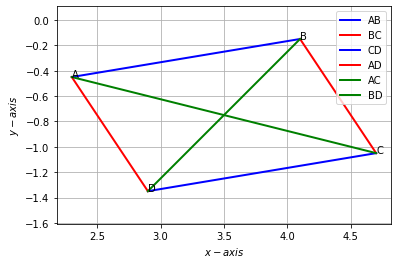
\includegraphics[width=\columnwidth]{parallelogram.png}
	\caption{Parallelogram}
\end{figure}

\end{enumerate}
\end{document}